\end{multicols}
\begin{multicols}{2}[\section{Technologies}]
\label{sec:technologies}

Since our design was heavily influenced by the technologies we wanted to use, we will give a brief discussion of the technologies we used and why we chose to use them.

We considered many technologies and looked at some of them intensively. Since we were building a web application we considered PHP, Ruby, Scala, pure Java and AspectJ as our main programming language. As the scheduler is a performance critical part of our application we dropped interpreted languages early. As we were all most familiar with Java and development tools for Java are widely available, we favored Java. We finally went with \ads{AspectJ}\link{http://www.eclipse.org/aspectj}{The eclipse AspectJ project}, which is built on top of Java, since it offers great flexibility through so called Aspects. It is tightly integrated in our favored IDE\footnote{Integrated Development Environment}, Eclipse, since it is an Eclipse project itself. We will discuss the use of Aspects within our application more in-depth later on.

As database backend we chose \ads{PostgreSQL}\link{http://www.postgresql.org/}{PostgreSQL} since it features strong adherence to the SQL standard and is the best open source implementation of \emph{referential integrity} in relational databases we knew of. Another strong argument for PostgreSQL was, that it allows for rich use of stored procedures, i.e. business logic within the database. As a matter of fact our application thus runs with PostgreSQL only, but could be ported to another database-engine easily, since only certain parts would have to be rewritten (PostgreSQL-specific parts within the data access layer and certain Aspects).

We used the standard web technologies like \ads{HTML}\link{http://www.w3.org/html/}{W3C HTML homepage} and \ads{CSS}\link{http://www.w3.org/Style/CSS/}{W3C Cascading StyleSheets homepage} in the front end. To keep things simple we stuck to related technologies which are all part of the \ads{XML family}, like \ads{XSL-T}\link{http://www.w3.org/TR/xslt}{XSL Transformations (XSLT)}. We will disucss the use of XML within our web application in the appropriate sections of this report.


\end{multicols}
\begin{multicols}{2}[\subsection{Libraries \& Frameworks}]
\label{sec:libraries-and-frameworks}

In order to enrich users experience, we made use of \ads{jQuery}\link{http://www.jquery.org}{Homepage of jQuery}. However, in order to keep the site accessible, we did not use it too much, i.e. the site should be fully functionial even if JavaScript was deactivated.

On the backend side we employed many libraries from the Apache Software Foundation, namely from their XML Software Stack. Amongst others, these are \ads{Apache Xalan}\link{http://xalan.apache.org}{Apache Xalan XSL-T Processor} and \ads{Apache FOP}\link{http://xmlgraphics.apache.org/fop/}{Apache XSL-FO Processor}, which we used to process XSL and generate not only XHTML, but also PDF files.

To create an easy to use installer we used \ads{IzPack}\link{http://www.izpack.org/}{Homepage of IzPack}. To make sure that our application works with different application servers it can optionally be bundled with Jetty\link{http://www.eclipse.org/jetty/}{Jetty Web Server} (an embedabble servlet container), which itself also is an Eclipse project.


\end{multicols}
\begin{multicols}{2}[\subsection{Tools}]
\label{sec:tools}

As mentioned in \autoref{sec:development-process}, we made use of a wiki and a ticket system. Both of them are contained in \ads{Trac}\link{http://trac.edgewall.org}{The Trac project}, a webinterface to \ads{Subversion}\link{http://subversion.tigris.org/}{Subversion homepage}, which we both used for source and version control.

We used \ads{JUnit}\link{http://www.junit.org/}{JUnit Test Driven Development} for writing unit tests. For the automatic execution of this, as well as generating reports about line coverage and branch coverage, we used \ads{Cobertura}\link{http://cobertura.sourceforge.net/}{Cobertura – Code coverage analysis tool}.

To build our project, we used GNU Make initially, but later on we switched to \ads{Apache Ant}, since it is more platform independent and features plugins which tightly integrate with AspectJ and JUnit. For testing purposes we employed \ads{Apache Tomcat}.

Regarding the versions of mentioned tools we followed the policy to include nothing more recent than the latest stable version of the Debian GNU/Linux distribution.


\end{multicols}
\begin{multicols}{2}[\subsection{Code generation toolbox}]
\label{sec:toolbox}

As we mentioned in \autoref{sec:architecture}, we did not want to maintain separate models for our database and our application. To achieve this technically we created an XML-file which represented an abstract description of our object-relational model. The syntax and semantics were defined using XML Schema\link{http://www.w3.org/XML/Schema}{XML Schema}. Using different XSL-T Stylesheets we automatically generated Java source files, an SQL install script, and documentation in XHTML.

As part of our build process we developed some tools for automatic generation of code. Basically the toolbox consists of several XSL-T stylesheets which can be used to create Java code, SQL scripts or XHTML documentation from a custom XML definitions file. This file contains the object-relational model and is specified using XML Schema.

The whole process of generating code is driven by Ant and part of our build process. Also the database can be easily set up using our toolchain.

\begin{figure}[H]
	\centering
		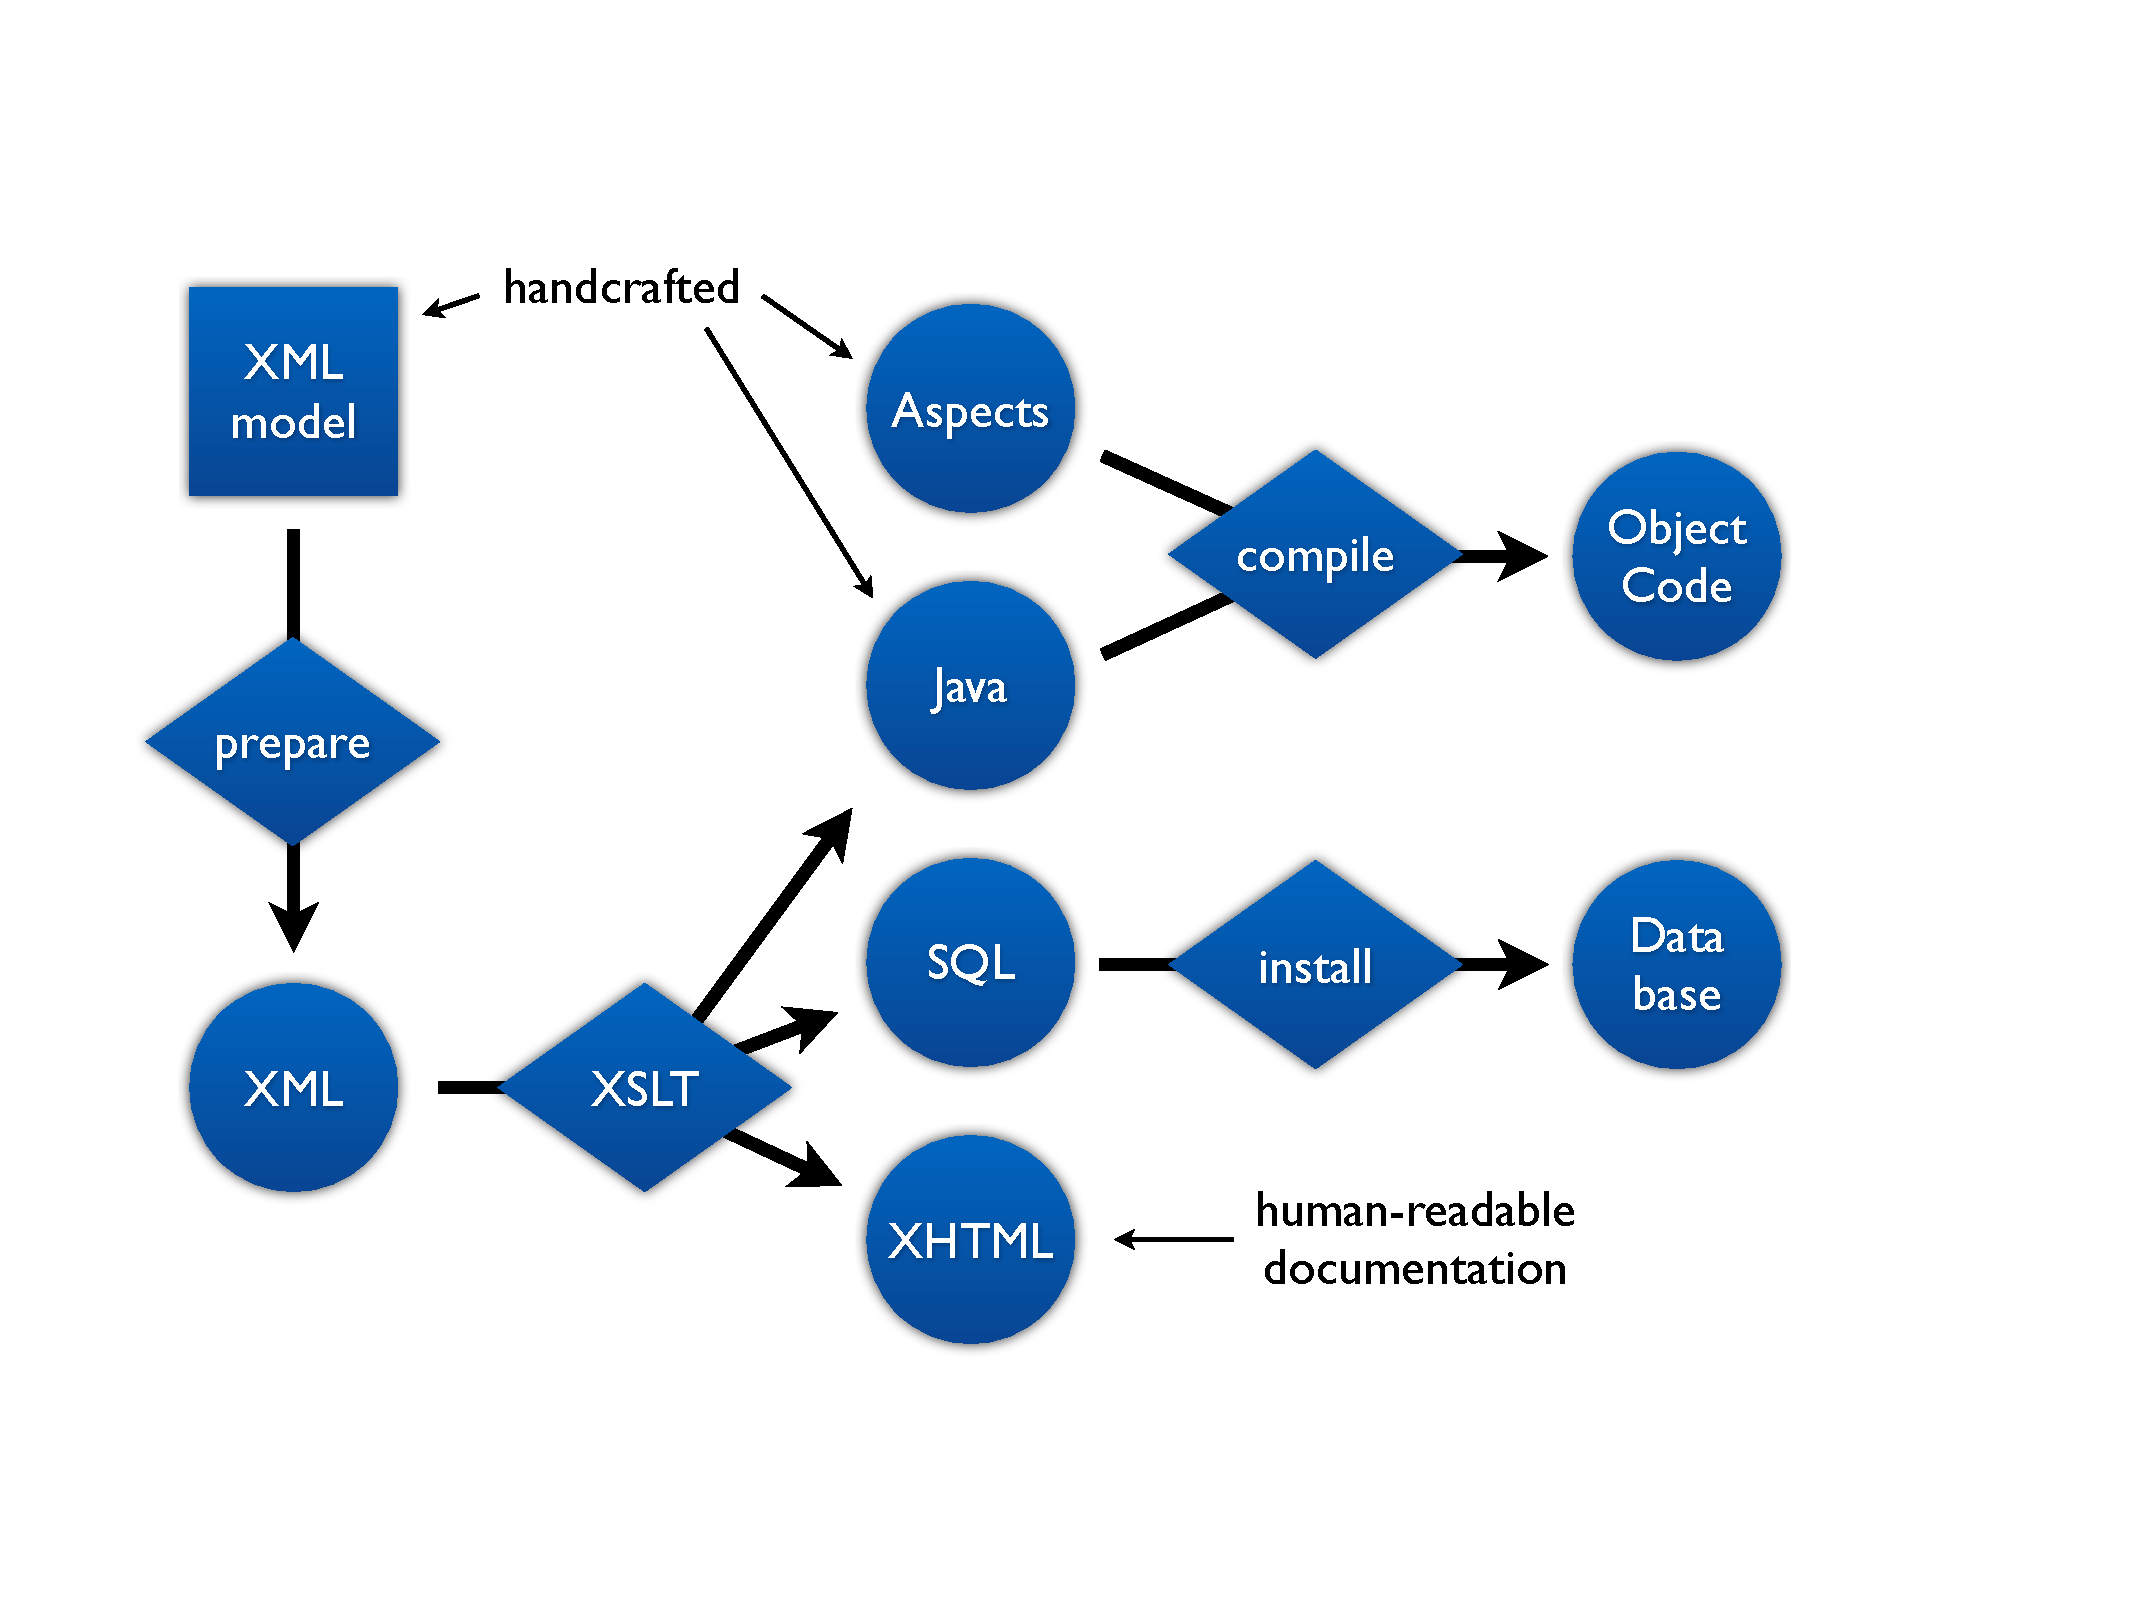
\includegraphics[width=\columnwidth]{images/build-process.pdf}
	\caption{The process of generating code within scetris.}
	\label{fig:build-process}
\end{figure}


